%-----------------------------------------------------------
%	Model formulation
%-----------------------------------------------------------
\subsection{Effective constitutive model form}
\subsubsection{Choosing the family of forms for effective constitutive model}

	To select the specific form, we will take the following key aspects into consideration:
\begin{enumerate}
\item Ability to accurately reproduce the response of a wide range of soft tissues and a wide range of deformations using the same form
\item Minimal number of parameters necessary
\item Minimal covariance between parameters
\item Minimal number of and computational cost of the constraints for convexity
\item Minimal computational demand
\end{enumerate}

    Using phenomenological approaches is necessary due to computational cost. The form of phenomenogical models for soft tissues generally falls into three families. The first family is composed of a summation of polynomials, 
%==========================================================%
%-------------------	begin EQUATION 	-------------------%
\begin{equation}
\begin{aligned}
\Psi	&= \sum_i\sum_j\sum_k c_{ijk}E_m^i E_n^j E_\phi^k. 
\end{aligned} \label{eqn:polynomialmodelform}
\end{equation}
%-------------------	 end EQUATION 	-------------------%
%==========================================================%
We will refer to this family as the polynomial series approach. The second family is composed of separated exponential functions of individual or combinations of invariants or strains used, for example by Vito \textit{et al.} \cite{vito_mechanical_1980},
%==========================================================%
%-------------------	begin EQUATION 	-------------------%
\begin{align}\label{eqn:vitomodelforms}
\Psi 	&= \sum_i\sum_j\sum_k c_{ijk} e^{b_{ijk}E_m^i E_n^j E_\phi^k}.
\end{align}
%-------------------	 end EQUATION 	-------------------%
%==========================================================%
We will refer to this family as the separated exponential approach. The final family is exponential models composed of a single exponential function of the sum of polynomials,
%==========================================================%
%-------------------	begin EQUATION 	-------------------%
\begin{equation}
\begin{aligned}\label{eqn:exponentialmodelform}
\Psi 	&= c_0 \left(e^{Q} - 1\right) \\
Q		&= \sum_i\sum_j\sum_k b_{ijk}E_m^i E_n^j E_\phi^k.
\end{aligned}
\end{equation}
%-------------------	 end EQUATION 	-------------------%
%==========================================================%
and we will refer to this family as the single exponential approach. 


\subsubsection{Generalized effective constitutive model form determination} \label{sec:possibleforms}

	Each approach (Eqn. \ref{eqn:polynomialmodelform}-\ref{eqn:exponentialmodelform}) has its own advantages and disadvantages. Polynomial series approach has the most flexibility. With sufficient number of terms, it can match any response perfectly, like Taylor series expansion. However, this family also requires large number of parameters, making parameter estimation and enforcing convexity very difficult. Polynomial series family is only convex in a specific range, extrapolating outside of this region is extremely unreliable. Even enforcing ellipticity and convexity inside of this region is actually much more costly than parameter estimation itself. The constrained optimization problem is not well pose. There are too many constraints and parameters that result in many local minima near or just outside of constrained region. No specific set of parameters are necessarily correct or better, but the objective function values are very similar. This leads to slow convergence and difficulties for most gradient based algorithms. As such, the polynomial series approach is not suitable for the effective constitutive model due to the slow parameter estimation. 


	The separated exponential approach generally suffers from the same issues as the polynomial series. This model form behaves like polynomial series with variable exponents, i.e. $c_1e^{b_1E_m} = c_1y^{b_1}$, where $y =e^{E_m}$. The advantage of this family of models is that similar and highly covariant terms such as $c_1 E_m + c_2 E_m^2 + c_3 E_m^3 ...$ can be avoided, reducing the number of parameters needed. However, like the polynomial series family, coupling terms such as $c_4 e^{b_4 E_m E_n}$ are not convex or elliptical functions, resulting in the same issues for parameter estimation and enforcing convexity. The number of parameters required to fully reproduce the mechanical response is still quite large. Moreover, for the same number of parameters, the separated exponential form is woefully insufficient at reproducing the mechanical response of soft tissues in comparison to the single exponential approach. As such, the advantages gained is actually quite minimal. 
    
    
    The single exponential approach has substantial parameter covariance, but is extremely effective at reproducing the response of soft tissues using a small number of parameters, is computationally efficient, and is easy to enforce convexity for. Because exponential function is monotonically increasing, enforcing convexity and ellipticity only requires the polynomial $Q$ to be convex and elliptical. This is the best balance for our goals (end of Section \ref{sec:straintensor}), and is thus our choice for the effective constitutive model. The first step is of course to examine the generalized Fung model (Eqn. \ref{eqn:exponentialmodelform}). We find that the generalized Fung model is not able to fully reproduce the mechanical response of pericardium and aortic valve tissues, it can only do so in a limited range. Although this is enough for most numerical simulations, where the deformations are generally limited to the physiologic range, it is not always sufficient for predicting the mechanical response when organs undergo significant changes in geometry, causing the deformations to change drastically. The easiest way to visualize this is through contour plots of the strain energy function (Fig. \ref{fig:strainenergycontours}). The mechanical response of soft tissues general has hyperelliptical contours (Fig. \ref{fig:strainenergycontours}A), whereas the generalized Fung model always has precisely elliptical contours (Fig. \ref{fig:strainenergycontours}B), which has some advantages. Ellipticity and convexity is very easy to guarantee, and the elasticity tensor and behavior at small strains is easy to derive. However, when the range of deformation is sufficiently large, the contours of the generalized Fung model essentially stretches and rotates to match the soft tissue to the best of its abilities (Fig. \ref{fig:strainenergycontours}B), but is not able to fully reproduce the resulting tissue response. It can only serve as an approximation.  


%%%%%%%%%%%%%%%%%%%%%%%%%%%%%%%%%%%%%%%%%%%%%%%%%%%%%%%%%%%%
%-------------------	begin FIGURE 	-------------------%
\begin{figure}
\centering
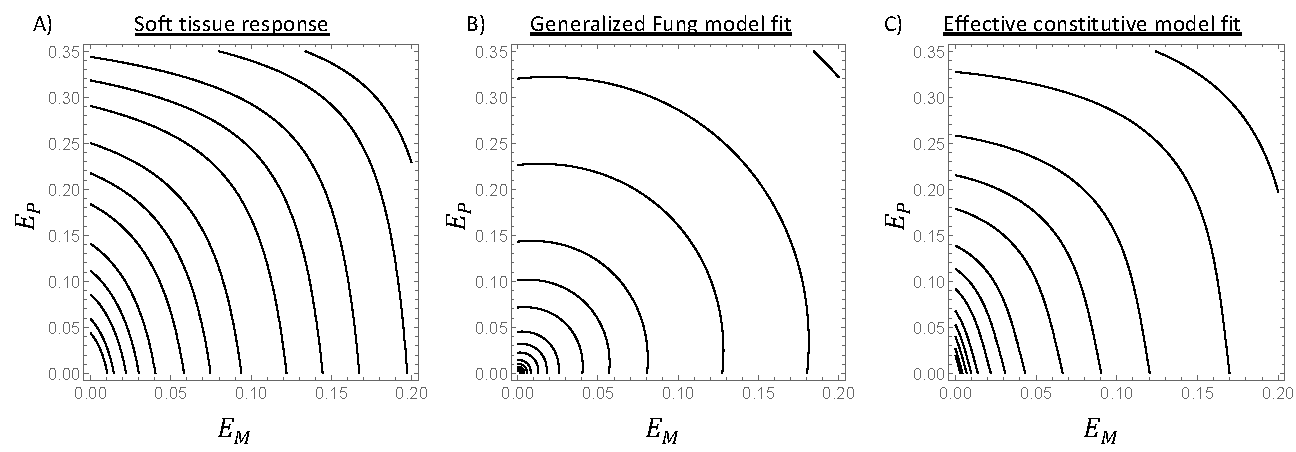
\includegraphics[width=6.5in]{Figures/strainenergycontours}
\caption{The contour plots of strain energy (kPa) of A) a bovine pericardial specimen using a meso-scale structural model \cite{zhang_modeling_2017}, B) best fit using the generalized Fung model (Eqn. \ref{eqn:generalizedfungmodel}), and C) best fit using the effective constitutive model we develop from herein showing the necessity of extending existence phenomenological model form.}
\label{fig:strainenergycontours}
\end{figure}
%-------------------	 end FIGURE 	-------------------%
%%%%%%%%%%%%%%%%%%%%%%%%%%%%%%%%%%%%%%%%%%%%%%%%%%%%%%%%%%%%

\subsubsection{Final effective material model form} \label{sec:finalform}

	Thus, for our effective constitutive model, we extended the polynomial $Q$ one step further, allowing hyperellipticity of the strain energy density function (Fig. \ref{fig:strainenergycontours}C). For the additional terms to include, we move up to the next even powers, up to the quartic terms (exponents $i+j+k\leq4$) (Eqn. \ref{eqn:exponentialmodelform}), as odd numbered powers do not yield elliptical functions. 
% The most generalized form possible is 
% %==========================================================%
% %-------------------	begin EQUATION 	-------------------%
% \begin{equation}
% \begin{aligned}\label{eqn:fullgeneralizeexponentialform}
% \Psi 	&= c_0 \left(e^{Q} - 1\right) \\
% Q		&= \sum_i\sum_j\sum_k b_{ijk} E_m^i E_n^j E_\phi^k, \quad  {i+j+k\leq4}.
% \end{aligned}
% \end{equation}
% %-------------------	 end EQUATION 	-------------------%
% %==========================================================%   
There is a total of 34 possible terms in Q. Not all terms are required or even admissible. Specifically, the following constraints are enforced on the model:
      
      \underline{Constraint 1}: \underline{The stress must be zero in the reference configuration}. Given that the stress is the gradient of $\Psi$, where is $\Psi^\prime = c_0 Q^\prime e^Q$, all terms that is non-zero in $Q^\prime$ at zero strain must be zero. This corresponds to all $i+j+k = 1$ terms, leaving 31 terms remaining. 
      
      \underline{Constraint 2}: \underline{The response must be elliptic}, that is the line joining any two point along the strain energy function surface must have positive curvature. Keeping in mind that the generalized Fung model (Eqn. \ref{eqn:exponentialmodelform}) is already close to being sufficient as reproducing the response of many soft tissues we tested. We only want to extend this to be able to reproduce a wide range of soft tissue responses. Furthermore, in considerations of limiting the number of parameters, reducing parameter correlation, non-elliptical terms making constrained optimization much more difficult, and that the non-elliptical terms must be small, we choose to forgo all $i+j+k = 3$ terms, leaving 21 terms remaining. 
      
      \underline{Constraint 3}: \underline{Response must be independent of the direction of shear}. Since we decompose the Green-Lagrange strain relative to the material axis, this creates a plane of symmetry in the soft tissue response for the direction of shear. Thus, the value of $E_\phi$ can only have even powers, $k = 2,4$. The following terms are thus necessarily zero: $E_m^3E_\phi$, $E_m^2E_nE_\phi$, $E_mE_n^2E_\phi$, $E_n^3E_\phi$, $E_mE_\phi^3$, $E_nE_\phi^3$, $E_mE_\phi$, and $E_nE_\phi$. 
      
The final form of the effective constitutive model is thus
%==========================================================%
%-------------------	begin EQUATION 	-------------------%
\begin{equation}
\begin{aligned}\label{eqn:generalizeexponentialform}
\Psi	=& c_0 \left(e^{Q} - 1\right) \\
Q		=& b_1 E_m^2 + b_2 E_n^2 + b_3 E_\phi^2 + b_4 E_m E_n + b_5 E_m^4 + b_6 E_n^4 + b_7 E_m^3 E_n + b_8 E_m^2 E_n^2 + b_9 E_m E_n^3	\\
	&+ b_{10} E_\phi^4 + b_{11} E_m^2E_\phi^2 + b_{12} E_n^2 E_\phi^2 + b_{13} E_m E_n E_\phi^2.
\end{aligned}
\end{equation}
%-------------------	 end EQUATION 	-------------------%
%==========================================================%








%-----------------------------------------------------------
%	Model convexity
%-----------------------------------------------------------
\subsubsection{Convexity and ellipticity}

	Perhaps the biggest advantage of the single exponential approach models is the convenience for enforcing ellipticity and convexity. Because ellipticity and convexity are preserved by monotonically increase functions, such as $e^x$, we only have to enforce ellipticity and convexity of $Q$ (Eqn. \ref{eqn:generalizeexponentialform}). Sylvester's criterion \cite{gilbert_positive_1991}, is the most convenient for constraints in this scenario, which is given by 
%==========================================================%
%-------------------	begin EQUATION 	-------------------%
\begin{equation}\label{eqn:convexitycriteria}
\begin{aligned}
\dpd[2]{Q}{E_m} \geq 0, \quad
\det
\begin{bmatrix}
\dpd[2]{Q}{E_m} & \dmd{Q}{2}{E_m}{}{E_n}{}\\
\dmd{Q}{2}{E_m}{}{E_n}{} & \dpd[2]{Q}{E_n}\\
\end{bmatrix} \geq0, \quad
\det
\begin{bmatrix}
\dpd[2]{Q}{E_m} & \dmd{Q}{2}{E_m}{}{E_n}{} & \dmd{Q}{2}{E_m}{}{E_\phi}{}\\
\dmd{Q}{2}{E_m}{}{E_n}{} & \dpd[2]{Q}{E_n} & \dmd{Q}{2}{E_n}{}{E_\phi}{}\\
\dmd{Q}{2}{E_m}{}{E_\phi}{} & \dmd{Q}{2}{E_n}{}{E_\phi}{} & \dpd[2]{Q}{E_\phi} \\
\end{bmatrix} \geq0.
\end{aligned}
\end{equation}
%-------------------	 end EQUATION 	-------------------%
%==========================================================%
\emph{This condition is also equivalent of strict convexity \cite{ball_strict_1980}}, so both conditions will be satisfied. For the generalized Fung model (Eqn. \ref{eqn:exponentialmodelform}), this simply required that $b_1>0$, $b_1b_2-b_4>0$, and $b_3(b_1b_2 - b_4^2) - b_5(b_2b_5 - b_4b_6) - b_6(b_1b_6 - b_4b5)>0$. Convexity and ellipticity for the effective constitutive model is also simple to enforce. The non-convex region start from a point along the respective axis for each component $E_m$, $E_n$, and $E_\phi$, then spreads out in the shape of a fan as the strain increases depending on which specific coupling terms, such as $E_m^3 E_n$ and $E_m E_n^3$ are present (Fig. \ref{fig:convexitybehavior}). As long as the effective constitutive model is convex on the largest value along the $E_m$, $E_n$, and $E_\phi$ axis respectively, then the effective constitutive model is convex over the entire range. For example, the effective constitutive model is convex if the maximum point on the $E_m$-axis is convex for $E_m^3 E_n$ (Fig. \ref{fig:convexitybehavior}A) or if the maximum point on the $E_n$-axis is convex for $E_m E_n^3$ (Fig. \ref{fig:convexitybehavior}B). Thus, assuming an upper limit of $E_m < 1$, $E_n < 1$, and $E_\phi < 1$, the following constraints on the parameters are sufficient to guarantee convexity and ellipticity,
%==========================================================%
%-------------------	begin EQUATION 	-------------------%
\begin{equation} \label{eqn:effmodelconstraints}
\begin{aligned}
b_1, b_2,b_3,b_5,b_6,b_{10} \geq 0	\\
4(b_1 + 6 b_5) (b_2 + b_8) - (b_4 + 3 b_7)^2 \geq 0		\\
4(b_2 + 6 b_6) (b_1 + b_8) - (b_4 + 3 b_9)^2 \geq 0 	\\
4(b_1 + b_{11}) (b_2 + b_{12}) - (b_{13} + b_4)^2 \geq 0 	\\
b_3+b_{11} \geq 0	\\
b_3+b_{12} \geq 0.	\\
\end{aligned}
\end{equation}
%-------------------	 end EQUATION 	-------------------%
%==========================================================%


%%%%%%%%%%%%%%%%%%%%%%%%%%%%%%%%%%%%%%%%%%%%%%%%%%%%%%%%%%%%
%-------------------	begin FIGURE 	-------------------%
\begin{figure}
\centering
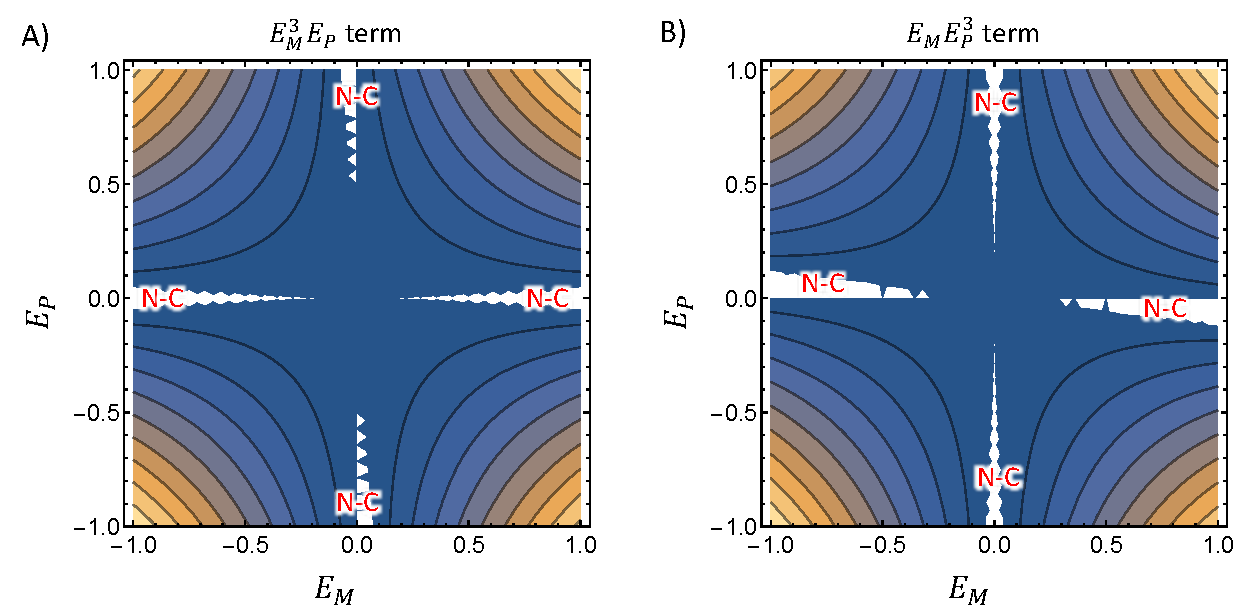
\includegraphics[width=6.5in]{Figures/convexitybehavior}
\caption{The criteria for ellipticity (Eqn. \ref{eqn:convexitycriteria}) plotted against the components of the Green-Lagrange strain for A) when including the $E_m^3E_n$ term and B) $E_mE_n^3$ term. The white regions are not convex (N-C), which start at a point along the axes and spreads out as the strain increases.}
\label{fig:convexitybehavior}
\end{figure}
%-------------------	 end FIGURE 	-------------------%
%%%%%%%%%%%%%%%%%%%%%%%%%%%%%%%%%%%%%%%%%%%%%%%%%%%%%%%%%%%%












